\documentclass[11pt]{article}
\usepackage[margin=1in]{geometry}
\usepackage{amsmath,amssymb,booktabs,graphicx,microtype}
\usepackage[hidelinks]{hyperref}
\usepackage{algorithm}
\usepackage{algpseudocode}
\usepackage[font=small]{caption}

\title{\vspace{-1.5em}A Decision-Focused Surrogate for AC Unit Commitment:\\
Learning the Linearisation Point and a Cardinality Cut}
\author{}
\date{}

\begin{document}\maketitle\vspace{-3em}

\section{Problem}

AC unit commitment (AC-UC) selects which generators run, $u\in\{0,1\}^{G}$, and
their output $p^g\in\mathbb{R}^{G}$, subject to the AC power-flow equations.
Because bus voltages enter through the products $V_iV_j$, the problem is a
nonconvex MINLP. On \texttt{case118} ($118$ buses, $54$ generators, $186$
branches) an exact spatial branch-and-bound solve takes $600$\,s.

\paragraph{The QCAC relaxation.} Constante-Flores and Li replace each voltage
product with its first-order expansion about a point $(V^{\mathrm{re}}_0,
V^{\mathrm{im}}_0)$ and absorb the residual in a slack $\xi\ge 0$ priced at
$\rho$. Writing the lifted variables $c_{ii}, c_{ij}, s_{ij}$ for
$|V_i|^2, \mathrm{Re}(V_iV_j^*), \mathrm{Im}(V_iV_j^*)$,
\begin{equation}
\bigl|\,c_{ii} - (2V^{\mathrm{re}}_{0,i}v^{\mathrm{re}}_i
+ 2V^{\mathrm{im}}_{0,i}v^{\mathrm{im}}_i - |V_{0,i}|^2)\,\bigr| \;\le\; \xi_i ,
\label{eq:lin}
\end{equation}
and analogously for $c_{ij},s_{ij}$. The expansion is accurate only near
$V_0$, so the published method \emph{iterates}: solve, re-linearise at the
solution, escalate $\rho$, repeat. On \texttt{case118} this converges in $3$--$4$
solves, each carrying all $54$ binaries, and reproduces the global optimum
($164{,}101.4$, $14$ units committed).

\paragraph{Goal.} Replace that loop with \emph{one continuous solve}.

\section{Method}

A network reads the instance parameters $x=(p^d,q^d)$ and emits two objects;
the solver then runs once.

\begin{equation}
x \;\longrightarrow\;
\underbrace{(V^{\mathrm{re}},V^{\mathrm{im}})}_{\text{linearisation point}}
\;,\;
\underbrace{[n_{\mathrm{lo}},\,n_{\mathrm{hi}}]}_{\text{cardinality cut}}
\end{equation}

\paragraph{Head 1: the linearisation point.} QCAC iterates \emph{in order to
find} this point, so predicting it removes the iteration. Its value is not
assumed: at the exact point, one continuous solve plus rounding recovers the
optimal commitment on $8/8$ instances ($-0.002\%$ gap, $100\%$ agreement) --
\emph{while $39.9$ of $54$ generators are still fractional}. Rounding is
therefore not the bottleneck; the linearisation point is.

\paragraph{Head 2: the cardinality cut.} The predicted point is never exact, and
that error is what costs money. The cut absorbs it:
\begin{equation}
n_{\mathrm{lo}} \;\le\; \textstyle\sum_{i} u_i \;\le\; n_{\mathrm{hi}},
\qquad
n_{\bullet} \;=\; n_{\min} + \Delta_{\bullet}(x),
\label{eq:cut}
\end{equation}
anchored on $n_{\min}$, the fewest generators that can meet the reserve
(largest capacity first). $n_{\min}$ needs no labels, costs a sort and a
cumulative sum, and is a \emph{valid} lower bound: the reserve cannot be served
with fewer. Measured over $112$ instances, $n^\star - n_{\min}\in[+6,+9]$ with
correlation $0.926$, so the head predicts one small, well-conditioned offset.

\paragraph{The cut must be hard.} This is the single most important
implementation detail. Imposed \emph{softly} -- as a penalty $\lambda\,\sigma$ on
the violation $\sigma$ -- the cut is inert whenever it binds: if it is violated
at the optimum, the penalty gradient in $u$ is the constant $\lambda$ and the
right-hand side $n_{\mathrm{hi}}$ \emph{drops out of the optimality conditions
entirely}. Empirically, replacing the learned band with $[0,0]$, or with
$[0,0]$ shifted by $-20$, reproduced its results bit-for-bit. We impose
\eqref{eq:cut} as a hard constraint, with a softly-priced fallback if that
renders an instance infeasible.

\begin{algorithm}[t]
\caption{Deployment: one continuous solve}\label{alg:deploy}
\begin{algorithmic}[1]
\State $(V,\,n_{\mathrm{lo}},n_{\mathrm{hi}}) \gets f_\theta(p^d,q^d)$
\State solve the QCAC relaxation linearised at $V$, with \eqref{eq:cut} hard and
       $u\in[0,1]^{G}$ \Comment{\emph{no} binaries}
\State $z \gets \mathbf{1}[u > 0.5]$
\State \textbf{reserve top-up:} switch on by descending $u$ until
       $p^{\max\!\top} z \ge (1+r)\sum p^d$
\State \textbf{upward repair:} while infeasible, commit the next-highest $u$
\State \textbf{downward repair:} for the least-confident committed units, try
       switching off; keep if feasible and cheaper
\State \Return $z$ and its AC dispatch
\end{algorithmic}
\end{algorithm}

\paragraph{Training.} Self-supervised on the deployment cost of
Algorithm~\ref{alg:deploy}; no optimal commitment enters the loss. Rounding
makes that cost piecewise constant in the network outputs, so there is no
pathwise derivative; we use an antithetic Gaussian smoothing estimator
\begin{equation}
\widehat{\nabla}_y J \;=\;
\frac{1}{P}\sum_{p=1}^{P}
\frac{J(y+\Sigma\epsilon_p)-J(y-\Sigma\epsilon_p)}{2}\,\Sigma^{-1}\epsilon_p ,
\qquad \epsilon_p\sim\mathcal{N}(0,I),
\end{equation}
with a \emph{per-group} $\Sigma$: the voltage outputs are $O(10^{-1})$ while the
cardinality bounds are measured in generators, $O(10)$. A common $\sigma$
perturbs the bound by a fraction of a unit, which can never change a rounded
commitment -- those coordinates then receive exactly zero signal.

\section{Implementation}

\paragraph{The relaxation is an SOCP; do not give it to a MINLP solver.}
Gurobi solves the \emph{continuous} QCAC relaxation -- which has no integer
variables -- by spatial branch-and-bound, because it will not certify
$c_{ij}^2+s_{ij}^2 \le c_{ii}c_{jj}$ as a rotated cone ($8$ of
\texttt{case118}'s $186$ remain bilinear). It reports \emph{``continuous model
is non-convex -- solving as a MIP''} and hits a $120$\,s limit. The same problem
is an SOCP: \textsc{Clarabel} solves it in $0.077$\,s, returning the same cost to
the digit at every $\rho\in[10^2,10^6]$ -- a $1200$--$2000\times$ difference, and
the difference between a trainable method and an untrainable one. Gurobi is
retained only where binaries genuinely exist (the reference solver).

\paragraph{The rank-1 cut is load-bearing.} Dropping
$c_{ij}^2+s_{ij}^2 \le c_{ii}c_{jj}$ makes the solve $158\times$ faster and the
slack still converges to $10^{-10}$, but the solution leaves the rank-1 manifold:
\texttt{case118} then returns $161{,}352.6$ against a proven optimum of
$164{,}101.4$ -- a cost \emph{below} the optimum, i.e.\ not physical. At zero
slack the linearisation only forces $c_{ii}$ to equal the first-order expansion
of $|V_i|^2$, not $|V_i|^2$ itself.

\paragraph{Instances.} One \emph{correlated} system-level draw per instance,
$s\sim U[0.80,1.15]$, with small per-bus jitter. An i.i.d.\ per-load factor --
the obvious choice -- averages out the aggregate variation that the reserve
constraint and merit order respond to: it gives under $1\%$ demand variation on
\texttt{case118} and $1$--$2$ distinct optimal commitments out of $32$. The
correlated draw gives ${\sim}10\%$ variation and $46$ distinct commitments over
$192$ instances (mean $14.7$ units committed).

\paragraph{Setup.} $192$ instances, $144$ train / $48$ held out. References from
QCAC iterative ($158$\,s each on average). The network is a two-layer SiLU trunk
($256$ wide) with a voltage head and a cardinality head; $v_{\text{scale}}=0.5$.
Training and evaluation use the \emph{same} restoration depth --- a mismatch
causes the network to compensate for a repair asymmetry that is absent at
evaluation time.

\section{Results}

Both cases run an \emph{identical} configuration: $K{=}1$ cardinality cut
imposed hard, 45 epochs, full batch, the same restoration depth in training and
evaluation, the same learning rate and perturbation scales, and a band
initialisation derived from $n_{\min}$ rather than chosen per case. Earlier runs
differed between the two grids, which makes any cross-case statement a tuning
artifact; nothing below does.

\begin{table}[h]\centering\small
\caption{Held-out instances, one continuous solve each. Identical restoration
and AC pricing for every arm --- only the source of the commitment differs.
\emph{Discrete} is the fraction of generators committed wrongly, \emph{continuous}
is $\|p^g-p^{g\star}\|_1/\sum p^{g\star}$ on the recovered dispatch, \emph{gap} is
true AC cost against the QCAC-iterative reference.}
\begin{tabular}{lcccc}
\toprule
\multicolumn{5}{l}{\textbf{\texttt{case118}} --- 192 instances, 144 train / 48 held out}\\
& labels & discrete & continuous & gap \\
\midrule
relaxation only (flat $V$, no cut) & --- & $40.32\%$ & $85.97\%$ & $+10.378\%$\\
NN proxy, supervised on $u^\star$ & \textbf{yes} & $3.32\%$ & $5.21\%$ & $+0.057\%$\\
NN proxy, self-supervised & no & $9.61\%$ & $12.61\%$ & $+0.242\%$\\
ours: $V$ only & no & $22.53\%$ & $23.34\%$ & $+3.319\%$\\
ours: $V$ + constant penalty & no & $4.17\%$ & $5.29\%$ & $+0.103\%$\\
\textbf{ours: $V$ + learned cardinality cut} & no & $\mathbf{4.05\%}$ & $5.92\%$ & $\mathbf{+0.049\%}$\\
\emph{control:} dummy band & no & $28.32\%$ & $51.50\%$ & $+6.718\%$\\
\emph{control:} random band & no & $38.43\%$ & $62.14\%$ & $+8.933\%$\\
\emph{control:} mean band (no per-instance information) & no & $5.63\%$ & $10.57\%$ & $+0.582\%$\\
\midrule
\multicolumn{5}{l}{\textbf{\texttt{case300}} --- 151 instances, 111 train / 40 held out}\\
\midrule
relaxation only (flat $V$, no cut) & --- & $26.52\%$ & $22.73\%$ & $+2.154\%$\\
NN proxy, supervised on $u^\star$ & \textbf{yes} & $1.63\%$ & $1.27\%$ & $-0.006\%$\\
ours: $V$ only & no & $24.57\%$ & $18.78\%$ & $+1.861\%$\\
ours: $V$ + constant penalty & no & $12.79\%$ & $9.10\%$ & $+0.592\%$\\
\textbf{ours: $V$ + learned cardinality cut} & no & $\mathbf{8.73\%}$ & $\mathbf{5.49\%}$ & $\mathbf{+0.296\%}$\\
\emph{control:} dummy band & no & $12.46\%$ & $7.49\%$ & $+0.626\%$\\
\emph{control:} random band & no & $15.04\%$ & $8.40\%$ & $+1.466\%$\\
\emph{control:} mean band (no per-instance information) & no & $9.60\%$ & $6.85\%$ & $+0.605\%$\\
\bottomrule
\end{tabular}
\end{table}

\paragraph{Headline.} One continuous solve reaches a $+0.049\%$ gap on
\texttt{case118} with $4.05\%$ of generators mis-committed, against $+10.378\%$
and $40.32\%$ for the same solve without the learned inputs --- $210\times$ on
gap, $10\times$ on discrete error. It also beats the \emph{supervised} NN proxy
($+0.057\%$), which trains on optimal commitments this method never sees, and
the self-supervised proxy by $4.9\times$. On \texttt{case300} the method reaches
$+0.296\%$ from a $+2.154\%$ relaxation, and is $2\times$ better than a constant
commitment penalty on all three measures.

\paragraph{The cut is learned, not a disguised constant.} Three controls, each
designed to refute the claim: a \emph{dummy} band (any always-violated value), a
\emph{random} band, and a \emph{mean} band --- the learned bounds averaged over
the test set, carrying no per-instance information. All fail on both cases; the
mean-band control, the sharpest of the three, loses by $12\times$ on
\texttt{case118} and $2.0\times$ on \texttt{case300}. The learned bounds vary
across instances with standard deviation $2.28$ and $2.19$ generators
respectively; a constant band has spread $0$.

\paragraph{Both heads are necessary.} $V$ alone gives $+3.319\%$ and $+1.861\%$.
The cut alone cannot help, because without a good expansion point the relaxation
is solved in the wrong place.

\paragraph{What did not work.} Three alternatives were measured and rejected
rather than tuned. \emph{Tiering:} splitting the fleet into $K$ merit-order tiers
and constraining each is worse at every setting --- $K{=}3$ interleaved
$+0.351\%$, random partition $+0.807\%$, contiguous merit blocks $+1.757\%$,
against $K{=}1$'s $+0.049\%$. \emph{A learned rounding threshold}
(L2O-MINLP's correction layer): a per-instance threshold ties the fixed $0.5$
exactly on \texttt{case118}, and the learned head moved to $0.499$--$0.500$ on
both cases, scoring identically to fixed rounding. \emph{Confidence-based
variable fixing:} helps only with a labelled $96.5\%$-accurate predictor; with
the label-free predictor ($9.6\%$ error) it worsens discrete error from $4.17\%$
to $7.68\%$ and makes $7$ of $48$ instances infeasible.

\begin{figure}[h]\centering
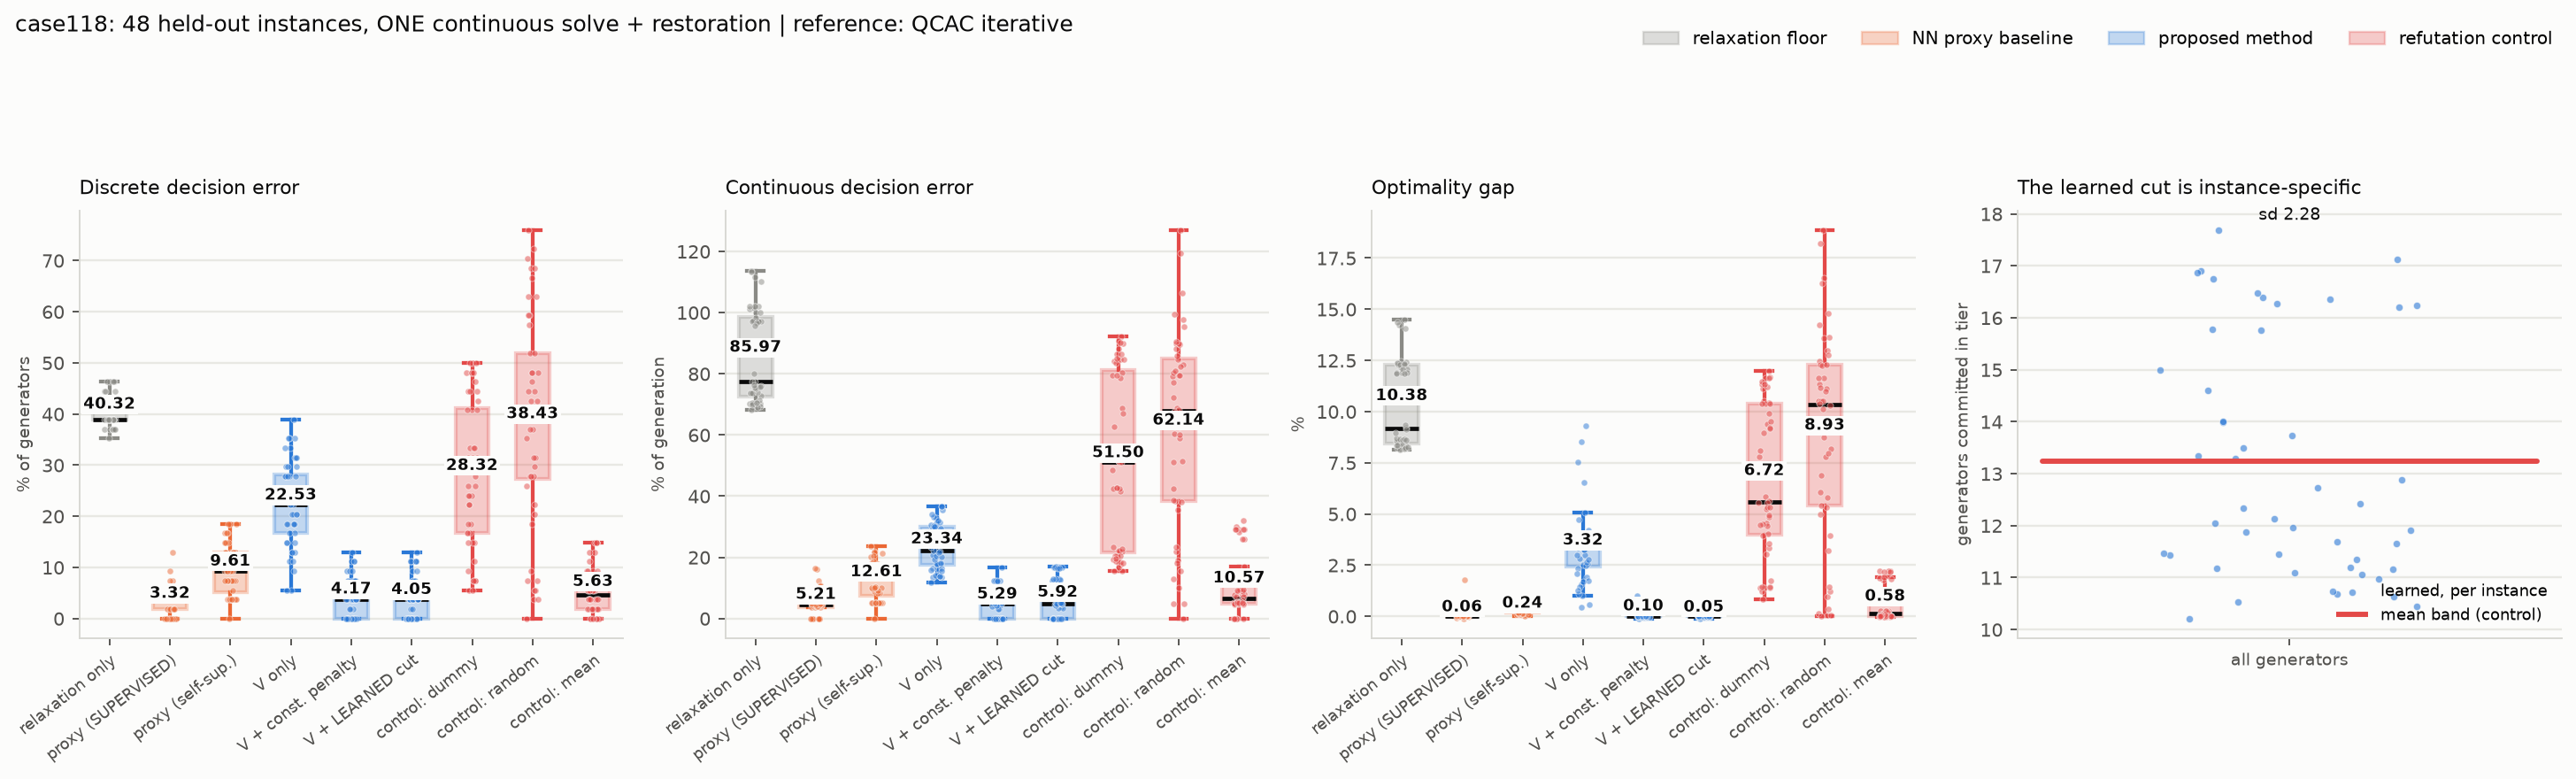
\includegraphics[width=\textwidth]{../results/FINAL_case118.png}
\caption{\texttt{case118}. The fourth panel is the claim itself: learned bounds
scattered per instance rather than collapsing onto the constant (red) that the
mean-band control uses.}
\end{figure}

\begin{figure}[h]\centering
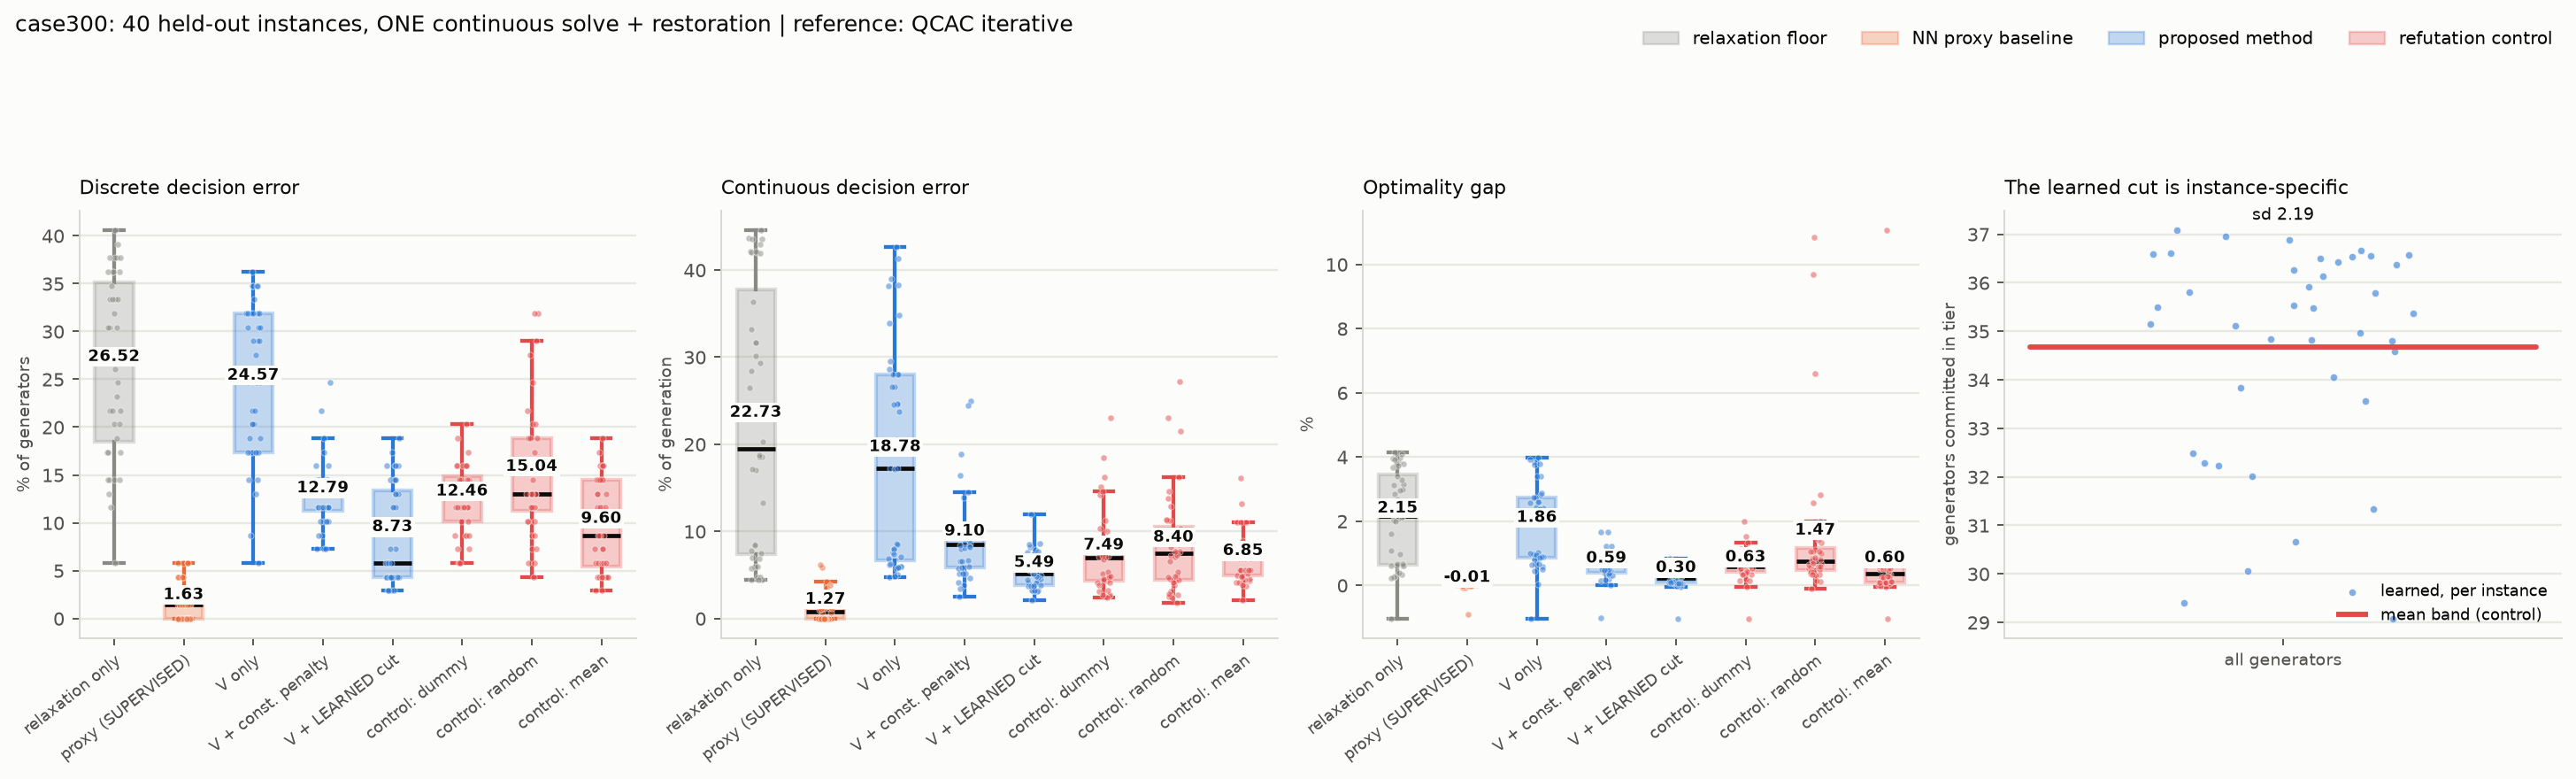
\includegraphics[width=\textwidth]{../results/FINAL_case300.png}
\caption{\texttt{case300}, same configuration. The supervised proxy is stronger
here; the learned cut still doubles the constant penalty on every measure.}
\end{figure}

\section{Limitations}

Results are stated relative to QCAC iterative, which reproduces the global
optimum where both were run but is not certified optimal everywhere --- in one
experiment this method beat it on $13$ of $24$ instances.

\texttt{case118} is at its ceiling: the oracle linearisation point, which no
method can beat, scores $-0.002\%$ against this method's $+0.049\%$. Further
gains there are not available.

\texttt{case300} is data-limited rather than method-limited. Its $V$ head
predicts a $600$-dimensional correction from $111$ training instances and
barely improves on the baseline alone ($+1.861\%$ versus $+2.154\%$); the
supervised proxy, which sees optimal commitments, reaches $-0.006\%$ there. The
price of those labels is one reference solve per training instance
($\approx 5$\,h for $111$), which this method does not pay.

Seed replication used re-splits of one instance pool, which is closer to
cross-validation than to independent replication.

\end{document}
